\documentclass[10pt,openright,twoside,french]{book}
\input philippe2013
\input philippe2013_activites
\pagestyle{empty}


\begin{document}

\TitreActivite{ii.1}{Modéliser des mesures}

À l'aide d'un ohmmètre, un ingénieur fait la mesure de la résistance $R$ aux bornes d'un radiateur électrique pour chacune des positions du bouton de commande (10 puissances possibles). Le tableau des valeurs de résistances (en ohms, arrondies à l'entier près) pour les différentes valeurs de puissances $P$ est donné ci-dessous.

\begin{center}
    \begin{tabular}{|>\bfseries c|*{10}{c|}}
        \hline
            Position bouton & 1 & 2 & 3 & 4 & 5 & 6 &7 & 8 & 9 & 10 \\
        \hline
            $P$ (en watts) & $200$ & $400$ & $600$ & $800$ & $\np{1000}$ & $\np{1200}$ & $\np{1400}$ & $\np{1600}$ & $\np{1800}$ & $\np{2000}$ \\
        \hline
            $R$ (en ohms) & $264$ & $132$ & $88$ & $66$ & $53$ & $44$ & $38$ & $33$ & $29$ & $26$ \\
        \hline
            \rule{0cm}{20pt} & & & & & & & & & & \\
        \hline
    \end{tabular}
\end{center}

\begin{enumerate}
    \item Dans le repère \Oij ci-dessous, placer les points de coordonnées $(P \pv R)$ pour chacun des couples donnés dans le tableau ($1~cm$ pour $200~W$ en abscisses et $1~cm$ pour $20~\Omega$ en ordonnées).
    \item Relier les points précédents pour représenter l'allure de la courbe représentative de la fonction qui à $P$ fait correspondre $R$.
    \item Cette courbe a la même allure que quelle autre courbe de fonction vue en seconde ? Quelle est le nom de ce type de courbe ?
    \item Dans la ligne vide du tableau, calculer pour chaque valeur $\sqrt{P \times R}$. Arrondir à l'unité près.
    \item Déduire une expression de $R$ en fonction de $P$ le plus possible en accord avec les résultats obtenus.
    \item Déterminer alors la valeur de résistance que devrait présenter le radiateur pour fournir une puissance de chauffe de $\np{3000}~W$.
\end{enumerate}
\begin{center}
    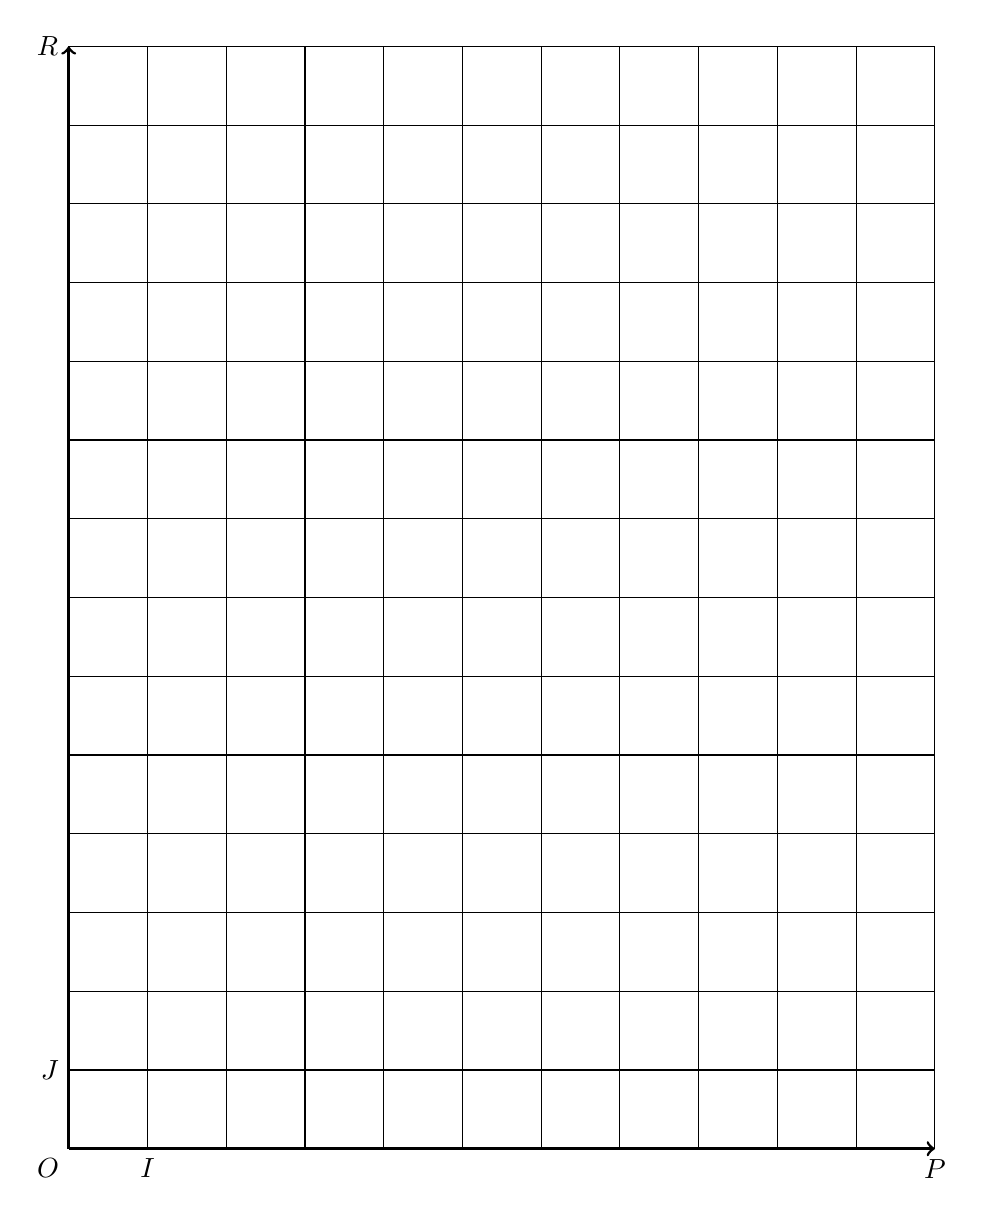
\begin{tikzpicture}[x=1cm,y=1cm]
        \draw[line width = 0.4pt] (0,0) grid[xstep=1,ystep=1] (11,14);
        \draw[line width = 1pt,->] (0,0) -- (11,0) node[below] {$P$};
        \draw[line width = 1pt,->] (0,0) -- (0,14) node [left] {$R$};
        \coordinate (O) at (0,0); \draw (O) node[below left] {$O$};
        \coordinate (I) at (1,0); \draw (I) node[below] {$I$};
        \coordinate (J) at (0,1); \draw (J) node[left] {$J$};
    \end{tikzpicture}
\end{center}


\end{document} 